\documentclass[aspectratio=169]{beamer}
\usepackage{will_handley_beamer}
\usepackage{pythonhighlight}
\usepackage{title_page}
\usetikzlibrary{positioning}
\usetikzlibrary{calc}
\usetikzlibrary{fit}

% Commands
% --------
% - \arxiv{arxiv number}
% - \cols{width}{lh column}{rh column}
% -  \begin{fig(left|right)}[fractional width (e.g 0.6) ]{name of image}
%        content of other column
%    \end{fig(left|right)}

% Talk details
% ------------
\title{\texttt{unimpeded} (\& other cosmological inference tools)}
%\subtitle{Marginal statistics and fully Bayesian forecasts}
\date{19\textsuperscript{th} October 2023}

\begin{document}

\begin{frame}
    \titlepage
\end{frame}
\begin{frame}
    \frametitle{Highlighted tools for this audience}
    \begin{enumerate}
        \item \texttt{anesthetic} \arxiv{1905.04768}
            \begin{itemize}
                \item how to get the most out of your nested sampling runs 
\item \texttt{\href{https://github.com/handley-lab/anesthetic}{github.com/handley-lab/anesthetic}}
            \end{itemize}
        \item \texttt{margarine} \arxiv{2207.11457}
            \begin{itemize}
                \item easy-to-use (neural) density estimation for marginal statistics
                \item \texttt{\href{https://github.com/htjb/margarine}{github.com/htjb/margarine}} 
            \end{itemize}
        \item \texttt{prescience} \arxiv{2309.06942}
            \begin{itemize}
                \item Fully Bayesian forecasts (no more need for Fisher)
                \item \texttt{\href{https://github.com/ThomasGesseyJones/FullyBayesianForecastsExample}{github.com/ThomasGesseyJones/FullyBayesianForecastsExample}} 
            \end{itemize}
        \item \texttt{unimpeded}
            \begin{itemize}
                \item up/downloading tool for transfering inference products (beyond chains)
                \item \texttt{\href{https://github.com/handley-lab/unimpeded}{github.com/handley-lab/unimpeded}} 
            \end{itemize}
    \end{enumerate}
\end{frame}

\begin{frame}
    \frametitle{Marginal inference}
    \begin{columns}
        \column{0.5\textwidth}
        \begin{itemize}
            \item Many cosmological likelihoods come with nuisance parameters that have limited relevance for onward inference.
            \item Notation: $\mathcal{L} = P(D|\theta,\alpha,M)$
                \begin{itemize}
                    \item[$\mathcal{L}$] Likelihood \hfill (e.g. \texttt{plik}),
                    \item[$D$] Data \hfill (e.g. CMB),
                    \item[$\theta$] Cosmological parameters \hfill (e.g. $\Omega_m$, $H_0$\ldots),
                    \item[$\alpha$] Nuisance parameters \hfill (e.g. $A_\text{planck}$\ldots),
                    \item[$M$] Model \hfill (e.g. $\Lambda$CDM).
                \end{itemize}
            \item Some marginal statistics (e.g. marginal means, posteriors\ldots) are easy to compute.
            \item More machinery is needed for e.g. nuisance marginalised likelihoods and marginal KL divergences $\mathcal{D}_\text{KL}$.
        \end{itemize}
        \column{0.5\textwidth}
        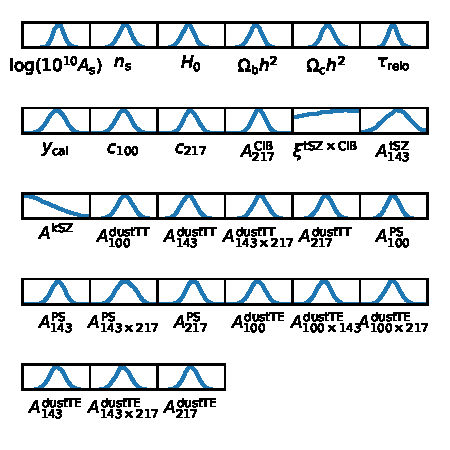
\includegraphics{figures/planck_2018_plik.pdf}
    \end{columns}
\end{frame}

\begin{frame}
    \frametitle{Relevant examples for this audience}
    \begin{enumerate}
        \item CMB
            \begin{itemize}
                \item Galatic foreground parameters: $A_i$, $n_i$,\ldots
                \item Calibration: $c$, $y$,\ldots
            \end{itemize}
        \item Gravitational wave events
            \begin{itemize}
                \item Nuisance event parameters: $M_1$, $M_2$, $\theta$, $\phi$, $r$, $z$, \ldots
            \end{itemize}
        \item (time-delay) supernovae
            \begin{itemize}
                \item Nuisance lens parameters: $\Phi_\text{lens}$
                \item Supernova systematics
            \end{itemize}
    \end{enumerate}
    \begin{itemize}
        \item Many modern cosmological problems present themselves in hierarchical form
        \item These (often well-studied) objects have a set of event-specific parameters $\alpha$ alongside  parameters of global interest $\theta$ (e.g. $H_0$).
        \item Ideally we would be able to have a ``nuisance marginalised'' likelihood for combining hierarchically.
    \end{itemize}
\end{frame}

\begin{frame}
    \frametitle{Nuisance marginalised likelihoods: Theory \arxiv{2207.11457}}
    \begin{columns}[t]
        \column{0.5\textwidth}
        \begin{itemize}
            \item Bayes theorem
                \begin{align}
                    \C[2]{\mathcal{L}}(\theta,\alpha) 
                    \times 
                    \C[1]{\pi}(\theta,\alpha) &= 
                    \C[0]{\mathcal{P}}(\theta,\alpha)
                    \times
                    \C[3]{\mathcal{Z}}\\
                    \C[2]{\text{Likelihood}}
                    \times
                    \C[1]{\text{Prior}}
                    &=
                    \C[0]{\text{Posterior}}
                    \times
                    \C[3]{\text{Evidence}}
                    \nonumber
                \end{align}
                \small{$\alpha$: nuisance parameters, $\theta$: cosmo parameters.}
            \item Marginal Bayes theorem
                \begin{equation}
                    \C[2]{\mathcal{L}}(\theta) 
                    \times 
                    \C[1]{\pi}(\theta) = 
                    \C[0]{\mathcal{P}}(\theta)
                    \times
                    \C[3]{\mathcal{Z}}
                \end{equation}
            \item Non-trivially gives \textbf{nuisance-free likelihood}
                \begin{equation}
                    \boxed{
                        \C[2]{\mathcal{L}}(\theta) 
                        = 
                        \frac{
                            \C[0]{\mathcal{P}}(\theta)
                            \C[3]{\mathcal{Z}}
                        }{
                            \C[1]{\pi}(\theta)
                        }
                    }
                    =
                    \frac{
                        \int \C[2]{\mathcal{L}}(\theta,\alpha) \C[1]{\pi}(\theta,\alpha) d{\alpha}
                    }
                    {
                        \int \C[1]{\pi}(\theta,\alpha) d{\alpha}
                    }
                \end{equation}
        \end{itemize}
        \column{0.5\textwidth}
        \textbf{Key properties}
        \begin{itemize}
            \item Given datasets $A$ and $B$, each with own nuisance parameters $\alpha_A$ and $\alpha_B$:
            \item If you use $\mathcal{L}_A(\theta)$, you get the same (marginal) posterior and evidence if you had run with nuisance parameters $\alpha_A$ (ditto $B$).
            \item If you run inference on $\mathcal{L}_A(\theta)\times\mathcal{L}_B(\theta)$, you get the same (marginal) posterior and evidence if you had run with all nuisance parameters $\alpha_A$, $\alpha_B$ on.
            \item[] \textit{(weak marginal consistency requirements on joint $\pi(\theta,\alpha_A,\alpha_B)$ and marginal priors)}
        \end{itemize}
    \end{columns}
\end{frame}

\begin{frame}
    \frametitle{Nuisance marginalised likelihoods: Practice}
    \student{harry_bevins}{Harry Bevins}{PhD$\to$JRF}
    \begin{columns}
        \column{0.6\textwidth}
        \begin{columns}
            \column{0.3\textwidth}
            \[
                \boxed{
                    \C[2]{\mathcal{L}}(\theta) 
                    = 
                    \frac{
                        \C[0]{\mathcal{P}}(\theta)
                        \C[3]{\mathcal{Z}}
                    }{
                        \C[1]{\pi}(\theta)
                    }
                }
            \]
            \column{0.7\textwidth}
            \begin{itemize}
                \item To compute the nuisance marginalised likelihood, need:
                    \begin{enumerate}
                        \item Bayesian evidence $\C[3]{\mathcal{Z}}$
                        \item Marginal prior and posterior densities
                    \end{enumerate}
            \end{itemize}
        \end{columns}
        \begin{enumerate}
            \item Use nested sampling to compute evidence $\C[3]{\mathcal{Z}}$ and marginal samples $\{\theta,\alpha\}_\mathcal{P}$ and $\{\theta,\alpha\}_\pi$.
            \item Use normalising flows to compute density estimators $\C[0]{\mathcal{P}(\theta)}$, $\C[1]{\pi(\theta)}$ from marginal samples.
        \end{enumerate}
        \begin{itemize}
            %\item Combination termed \texttt{margarine} \arxiv{2205.12841}
            \item Emulators usually much faster than original likelihoods
            \item Library of pre-trained bijectors to be used as priors/emulators/nuisance marginalised likelihoods
            \item e.g. easy to apply a \textit{Planck}/DES/HERA/JWST prior or likelihood to your existing MCMC chains without needing to install the whole cosmology machinery.
        \end{itemize}

        \column{0.4\textwidth}
        \begin{tikzpicture}[
                rednode/.style={rectangle, draw=red!60, fill=red!5, very thick, minimum size=5mm},
                bluenode/.style={rectangle, draw=blue!60, fill=blue!5, very thick, minimum size=5mm},
                greennode/.style={rectangle, draw=green!60, very thick, minimum size=5mm},
                node distance=0.5cm,
                remember picture, overlay
            ]
            \node<1->[bluenode, xshift=0.5\textwidth, yshift=-0.25\textwidth](likelihood) at (current page.north)  {$ \mathcal{L}(\theta,\alpha)$};
            \node<1->[bluenode, right = of likelihood.east](prior) {$ \pi(\theta,\alpha)$};

            \coordinate<1-> (likelihoodprior) at ($(likelihood.south)!0.5!(prior.south)$);

            \node<2->[rednode, below = of likelihoodprior](nestedsampling) {Nested Sampling};
            \draw<2->[->](likelihood.south) -- (likelihood|-nestedsampling.north);
            \draw<2->[->](prior.south) -- (prior|-nestedsampling.north);

            \node<3->[bluenode, below = of nestedsampling](posterior) {$ \{\theta,\alpha\}_\mathcal{P}$};
            \draw<3->[->](nestedsampling.south-|posterior) -- (posterior.north);
            \node<4->[bluenode, left = of posterior.west](evidence) {$ \mathcal{Z}$};
            \draw<4->[->](nestedsampling.south-|likelihood) -- (evidence.north);
            \node<5->[bluenode, right = of posterior.east](priorSamples) {$ \{\theta,\alpha\}_\pi$};
            \draw<5->[->](nestedsampling.south-|prior) -- (priorSamples.north);

            \coordinate<5-> (posteriorprior) at ($(posterior.south)!0.5!(priorSamples.south)$);

            \node<6->[rednode, below = of posteriorprior](margarine)  {Density Estimation};

            \draw<6->[->](posterior.south) -- (margarine.north-|posterior.east);
            \draw<6->[->](priorSamples.south) -- (margarine.north-|priorSamples.west);

            \node<7->[bluenode, below = of posterior|-margarine.south](marginalPosterior) {$ \mathcal{P}(\theta)$};


            \draw<7->[->](margarine.south-|marginalPosterior.east) -- (marginalPosterior.north);


            \node<8->[bluenode, below = of marginalPosterior.south-|margarine.south-|priorSamples](marginalPrior) {$ \pi(\theta)$};
            \draw<8->[->](margarine.south-|priorSamples.west) -- (marginalPrior.north);


            \node<9->[bluenode, below = of marginalPosterior](marginalLikelihood) {$ \mathcal{L}(\theta)$};


            \draw<9->[->](evidence.south) -- (marginalLikelihood.west);
            \draw<9->[->](marginalPosterior.south) -- (marginalLikelihood.north);
            \draw<9->[->](marginalPrior.west) -- (marginalLikelihood.east);

            \node<10->[greennode,behind path,fit=(nestedsampling) (marginalPosterior) (priorSamples) (evidence),] {};

        \end{tikzpicture}
    \end{columns}
\end{frame}

\begin{frame}
    \frametitle{Combination}
    \begin{columns}
        \column{0.5\textwidth}
%\begin{tikzpicture}[squarednodeA/.style={rectangle, draw=red!60, fill=red!5, very thick, minimum size=5mm},
%squarednodeB/.style={rectangle, draw=blue!60, fill=blue!5, very thick, minimum size=5mm},
%squarednodeC/.style={rectangle, draw=green!60, fill=green!5, very thick, minimum size=5mm}]
%
%\node[squarednodeA, text width=3cm, align=center](inference3) at (17, -1.5) {Nested Sampling with $\theta$, $\alpha_A$ and $\alpha_B$};
%
%\node[squarednodeB](fulllikelihood1) at (15, 1.5){$ \mathcal{L}_A(\theta,\alpha_A)$};
%\node[squarednodeB](fulllikelihood2) at (16.85, 1.5){$ \mathcal{L}_B(\theta,\alpha_B)$};
%\node[squarednodeB](fulljointlikelihood) at (16, 0){$ \mathcal{L}_A(\theta,\alpha_A) \mathcal{L}_B(\theta,\alpha_B)$};
%\node[squarednodeB](fullprior) at (19, 1.5){$ \pi_{AB}(\theta,\alpha_A, \alpha_B)$};
%
%\draw[->](fulllikelihood1.south) -- (15.5, 0.3);
%\draw[->](fulllikelihood2.south) -- (16.5, 0.3);
%\draw[->](fullprior.south) -- (inference3.north);
%\draw[->](fulljointlikelihood.south) -- (inference3.north);
%
%\node[squarednodeB](jointEvidence2) at (15, -3){$ \mathcal{Z}_{AB}$};
%\node[squarednodeB](jointPosterior2) at (17, -3){$ \{\theta\}_{\mathcal{P}_{AB}}$};
%
%\draw[<-](jointEvidence2.north) -- (16, -2);
%\draw[<-](jointPosterior2.north) -- (inference3.south);
%
%\node[squarednodeB](jointPosteriorNuisance) at (19, -3){$ \{\alpha_A, \alpha_B\}_{\mathcal{P}_{AB}}$};
%\draw[->](18, -2) -- (jointPosteriorNuisance.north);
%\draw[blue,thick](16.2, -3.5) -- (20.1, -3.5) -- (20.1, -2.5) -- (16.2, -2.5) -- (16.2, -3.5);
%
%\end{tikzpicture}

        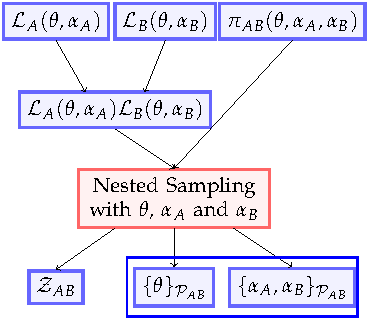
\includegraphics[width=0.7\textwidth]{figures/full_margarine.pdf}

        \column{0.5\textwidth}
%\begin{tikzpicture}[squarednodeA/.style={rectangle, draw=red!60, fill=red!5, very thick, minimum size=5mm},
%squarednodeB/.style={rectangle, draw=blue!60, fill=blue!5, very thick, minimum size=5mm},
%squarednodeC/.style={rectangle, draw=green!60, fill=green!5, very thick, minimum size=5mm}]
%
%\node[squarednodeB](likelihood1) at (6, 1.5){$ \mathcal{L}_A(\theta,\alpha_A)$};
%\node[squarednodeB](prior1) at (8, 1.5){$ \pi_A(\theta,\alpha_A)$};
%
%\node[squarednodeC, text width=3cm, align=center](NestedMarg1) at (7, 0){Nested Sampling + \textsc{Margarine}};
%
%\draw[->](likelihood1.south) -- (6, 0.5);
%\draw[->](prior1.south) -- (8, 0.5);
%
%\node[squarednodeB](marglike1) at (6, -1.5){$ \mathcal{L}_A(\theta)$};
%\node[squarednodeB](margprior1) at (9, -1.5){$ \pi(\theta)$};
%
%\draw[->](6, -0.5) -- (6, -1.2);
%\draw[->](8, -0.5) -- (9, -1.2);
%
%\node[squarednodeB](likelihood2) at (10, 1.5){$ \mathcal{L}_B(\theta,\alpha_B)$};
%\node[squarednodeB](prior2) at (12, 1.5){$ \pi_B(\theta,\alpha_B)$};
%
%\draw[->](likelihood2.south) -- (10, 0.5);
%\draw[->](prior2.south) -- (12, 0.5);
%
%\node[squarednodeC, text width=3cm, align=center](NestedMarg1) at (11, 0){Nested Sampling + \textsc{Margarine}};
%
%\node[squarednodeB](marglike2) at (12, -1.5){$ \mathcal{L}_B(\theta)$};
%\draw[->](12, -0.5) -- (12, -1.2);
%\draw[->](10, -0.5) -- (9, -1.2);
%
%\node[squarednodeB](combinedlike) at (7, -3){$ \mathcal{L}_A(\theta) \mathcal{L}_B(\theta)$};
%
%\draw[->](marglike1.south) -- (combinedlike.north);
%\draw[->](marglike2.south) -- (combinedlike.north);
%
%\node[squarednodeA, text width=3cm, align=center](inference2) at (9, -4.5) {Nested Sampling with $\theta$};
%
%\draw[->](combinedlike.south) -- (8, -4);
%\draw[->](margprior1.south) -- (10, -4);
%
%\node[squarednodeB](jointEvidence) at (8, -6){$ \mathcal{Z}_{AB}$};
%\node[squarednodeB](jointPosterior) at (10, -6){$ \{\theta\}_{\mathcal{P}_{AB}}$};
%
%\draw[->](8, -5) -- (jointEvidence.north);
%\draw[->](10, -5) -- (jointPosterior.north);
%\end{tikzpicture}
        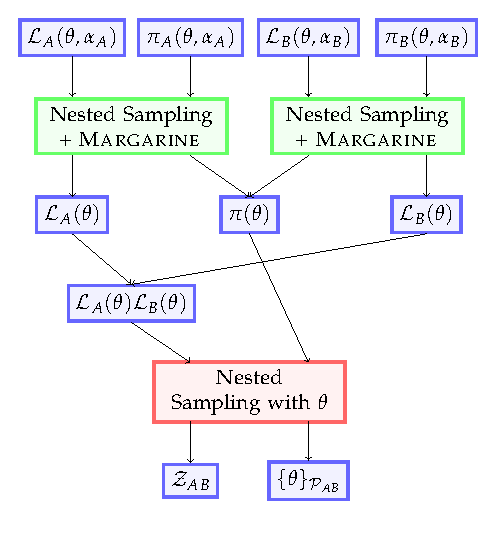
\includegraphics[width=0.9\textwidth]{figures/quick_margarine.pdf}
        
    \end{columns}
\end{frame}

\begin{frame}
    \frametitle{History of margarine}
    \begin{itemize}
        \item Papamakarios et al \arxiv{1912.02762} (normalising flows)
        \item Alsing et al \arxiv{1903.00007} (Delfi)
        \item Nested sampling with any prior you like (Alsing \& Handley) \arxiv{2102.12478}
        \item \texttt{margarine} (theory) Bevins et al \arxiv{2207.11457}
        \item \texttt{margarine} (practice) Bevins et al \arxiv{2205.12841}
    \end{itemize}

\end{frame}

\begin{frame}[fragile]
    \frametitle{\texttt{unimpeded}}
    \framesubtitle{Universal Model comparison and Parameter Estimation Distributed over Every Dataset}
    \student{dily_ong}{Dily Ong}{PhD}
    \begin{columns}
        \column{0.5\textwidth}
    \begin{itemize}
        \item Python tool for seamlessly downloading, uploading and cacheing of chains
        \item Data stored on \texttt{zenodo} 
        \item hdf5 storage for fast \& reliable storage
        \item \texttt{anesthetic} compatible for processing of chains~\arxiv{1905.04768}
        \item $\alpha$-testers wanted! (email \href{mailto:wh260@cam.ac.uk}{wh260@cam.ac.uk}) 
        \item End goal -- community library which everyone contributes to so expensive inference products are reusable and reused.
    \end{itemize}
        \column{0.5\textwidth}


\lstset{language=Python}
\lstset{frame=lines}
\lstset{basicstyle=\footnotesize}
\begin{lstlisting}
from unimpeded import Unimpeded
store = Unimpeded(cache='data.hdf5')
samps = store('planck')
samps.H0.plot.kde_1d()
samps = store('planck', model='klcdm')
samps.H0.plot.kde_1d()
\end{lstlisting}
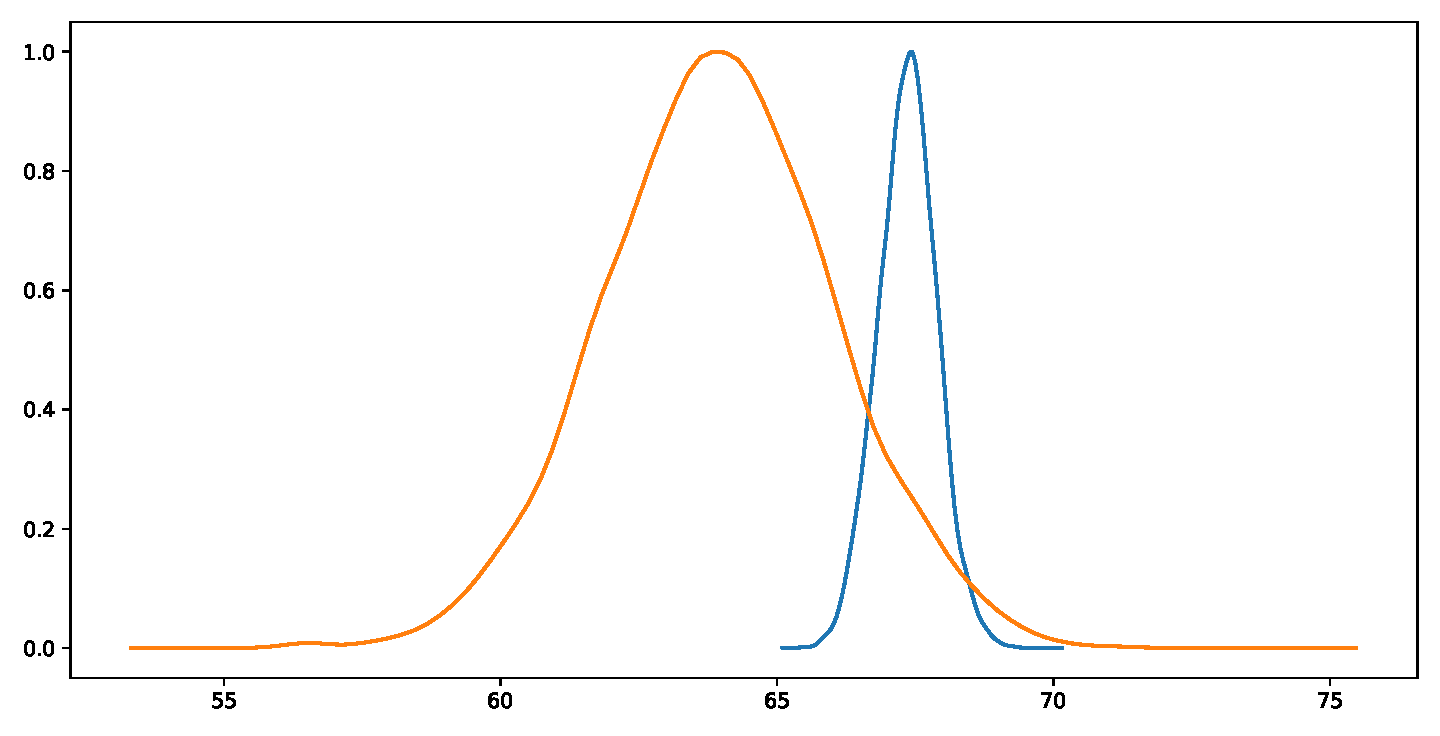
\includegraphics[width=\textwidth]{figures/unimpeded.pdf}

        
    \end{columns}
\end{frame}
 

\begin{frame}
    \frametitle{Inference Legacy Archive}
    \begin{columns}
        \column{0.5\textwidth}
        \begin{itemize}
            \item DiRAC 2020 RAC allocation of 30MCPUh
            \item Main goal: Planck Legacy Archive equivalent
            \item Parameter estimation $\to$ Model comparison
            \item MCMC $\to$ Nested sampling
            \item Planck $\to$ $\{\text{Planck}, \text{DESY1}, \text{BAO}, \ldots \}$
            \item Pairwise combinations
            \item Suite of tools for processing these 
                \begin{itemize}
                    \item \texttt{anesthetic} $2.0$
                    \item \texttt{unimpeded} $1.0$
                    \item \texttt{zenodo} archive
                    \item \texttt{margarine}
                \end{itemize}
            \item MCMC chains also available.
            \item Library of bijectors emulators for fast re-use
        \end{itemize}
        \column{0.5\textwidth}
        
\includegraphics[width=\textwidth]{logos/dirac}
        \includegraphics[width=0.5\textwidth,page=21]{figures/himmelblau}%
        \includegraphics[width=0.5\textwidth,page=15]{figures/himmelblau}
    \end{columns}
\end{frame}

\begin{frame}
    \frametitle{Cosmological forecasting}
    \student{thomas_gessey-jones}{Thomas Gessey-Jones}{PhD}
    \framesubtitle{Have you ever done a Fisher forecast, and then felt Bayesian guilt?}
    \vspace{-20pt}
    \begin{columns}[t]
        \column{0.5\textwidth}
        \begin{itemize}
            \item Cosmologists are interested in forecasting what a Bayesian analysis of future data might produce.
            \item Useful for:
                \begin{itemize}
                    \item white papers/grants,
                    \item optimising existing instruments/strategies,
                    \item picking theory/observation to explore next.
                \end{itemize}
            \item To do this properly:
                \begin{enumerate}
                    \item start from current knowledge $\pi(\theta)$, derived from current data
                    \item Pick potential dataset $D$ that might be collected from $P(D)\: (=\mathcal{Z})$
                    \item Derive posterior $P(\theta|D)$
                    \item Summarise science (e.g. constraint on $\theta$, ability to perform model comparison)
                \end{enumerate}
        \end{itemize}

        \column{0.5\textwidth}
        \begin{itemize}
            \item This procedure should be marginalised over:
                \begin{enumerate}
                    \item All possible parameters $\theta$ (consistent with prior knowledge)
                    \item All possible data $D$
                \end{enumerate}
            \item i.e. marginalised over the joint $P(\theta,D)=P(D|\theta)P(\theta)$.
            \item Historically this has proven very challenging.
            \item Most analyses assume a fiducial cosmology $\theta_*$, and/or a Gaussian likelihood/posterior (c.f. Fisher forecasting).
            \item This runs the risk of biasing forecasts by baking in a given theory/data realisation.
        \end{itemize}
        
    \end{columns}

\end{frame}


\begin{frame}
    \frametitle{Fully Bayesian Forecasting~\arxiv{2309.06942}}
    \student{thomas_gessey-jones}{Thomas Gessey-Jones}{PhD}
    \begin{columns}
        \column{0.5\textwidth}
        \begin{itemize}
            \item Simulation based inference gives us the language to marginalise over parameters $\theta$ and possible future data $D$.
            \item Evidence networks~\arxiv{2305.11241} give us the ability to do this at scale for forecasting.
            \item Demonstrated in 21cm global experiments, marginalising over:
                \begin{itemize}
                    \item theoretical uncertainty
                    \item foreground uncertainty
                    \item systematic uncertainty
                \end{itemize}
            \item Able to say ``at 67mK radiometer noise'', have a 50\% chance of 5$\sigma$ Bayes factor detection.
            \item Can use to optimise instrument design
            \item Re-usable package: \texttt{prescience}
        \end{itemize}
        \column{0.5\textwidth}
        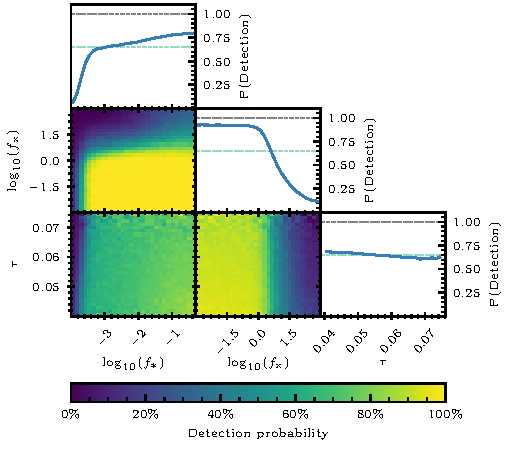
\includegraphics[width=\textwidth]{figures/fbf.pdf}
    \end{columns}
\end{frame}

\begin{frame}
    \frametitle{Conclusions}
    \framesubtitle{\href{https://www.github.com/handley-lab}{github.com/handley-lab}}
    \tikz[overlay,remember picture]
        \node[anchor=north east] (A) at ($(current page.north east)+(0,0)$) {
            
\includegraphics[width=0.1\textheight]{figures/students/adam_ormondroyd.jpg}%
            %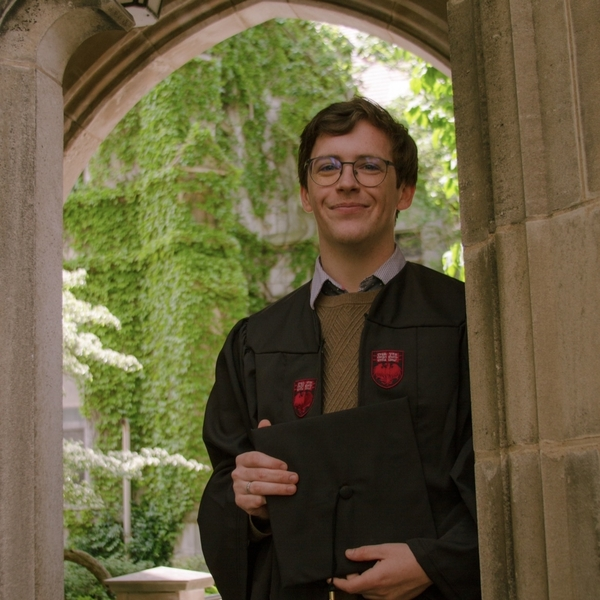
\includegraphics[width=0.1\textheight]{figures/students/cole_meldorf.jpg}%
            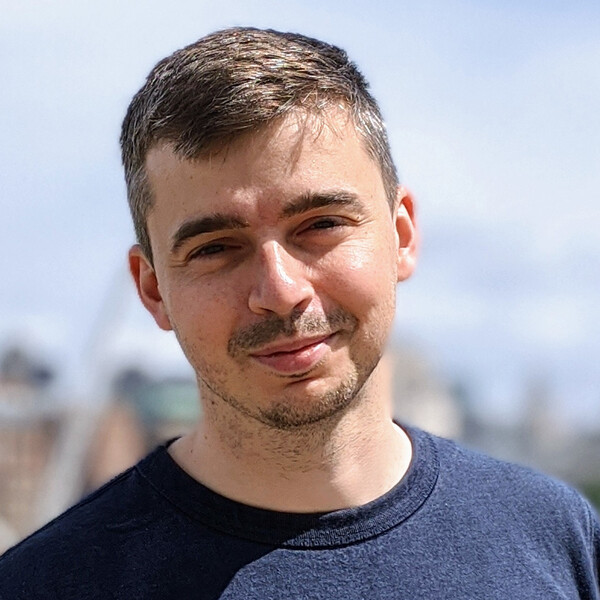
\includegraphics[width=0.1\textheight]{figures/students/david_yallup.jpg}%
            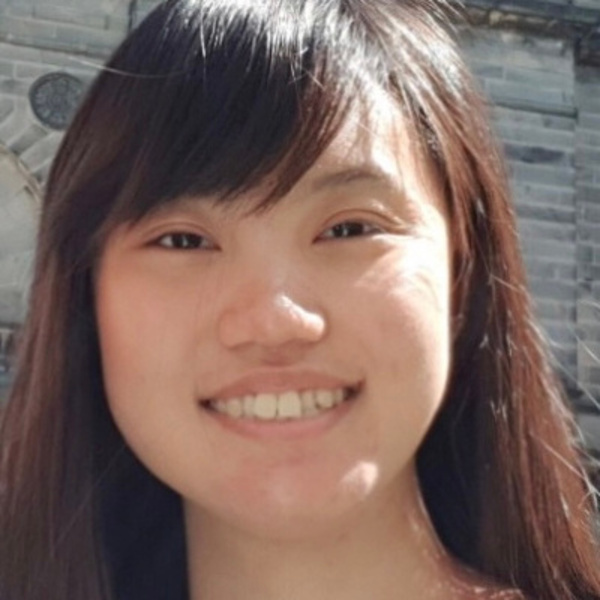
\includegraphics[width=0.1\textheight]{figures/students/dily_ong.jpg}%
            %
\includegraphics[width=0.1\textheight]{figures/students/harry_bevins.jpg}%
            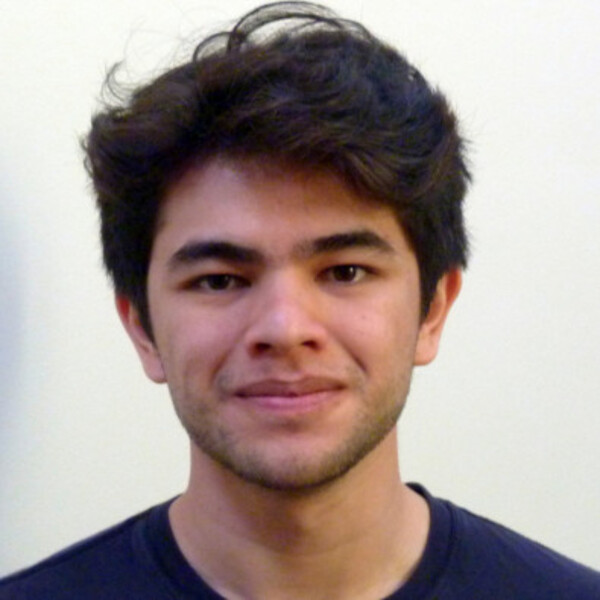
\includegraphics[width=0.1\textheight]{figures/students/ian_roque.jpg}%
            
\includegraphics[width=0.1\textheight]{figures/students/george_carter.jpg}%
            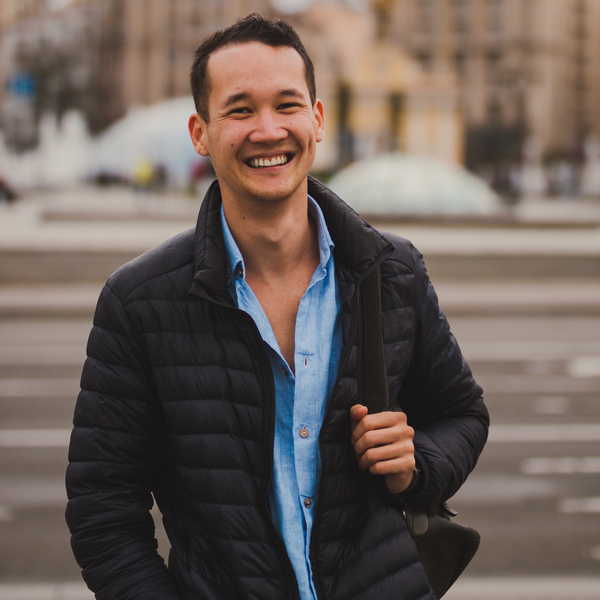
\includegraphics[width=0.1\textheight]{figures/students/kilian_scheutwinkel.jpg}%
            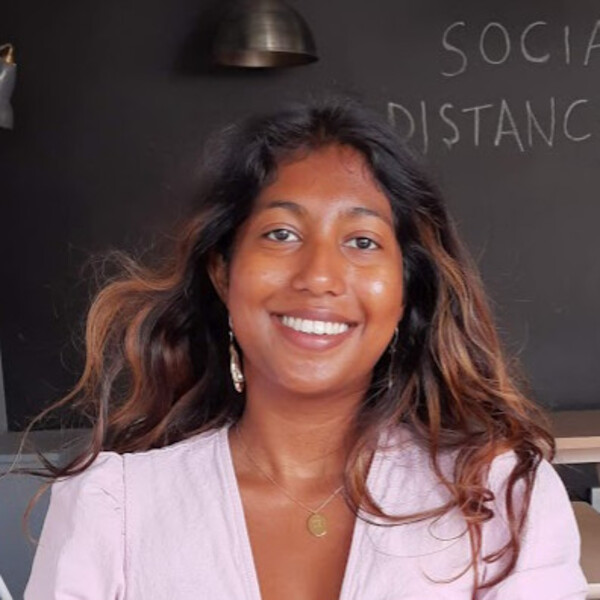
\includegraphics[width=0.1\textheight]{figures/students/metha_prathaban.jpg}%
            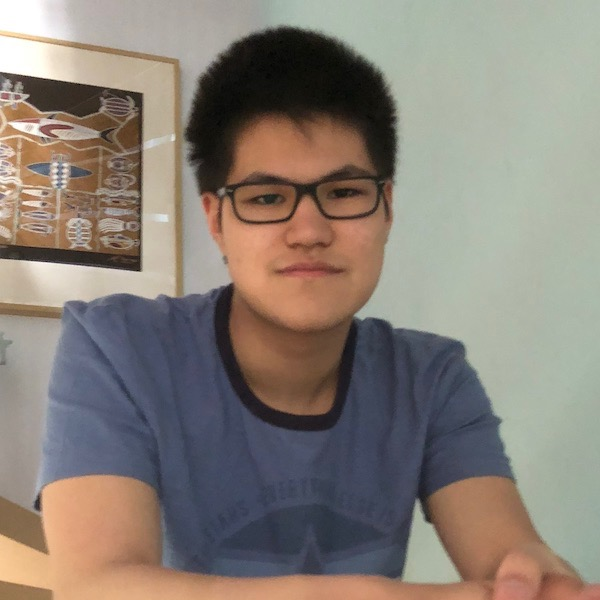
\includegraphics[width=0.1\textheight]{figures/students/namu_kroupa.jpg}%
            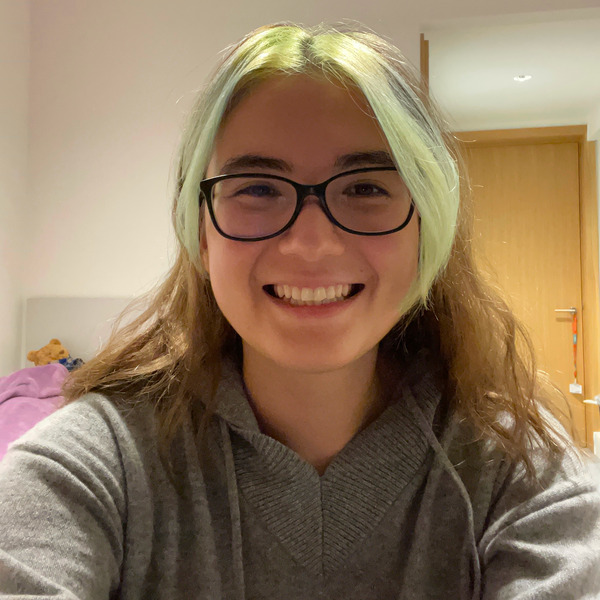
\includegraphics[width=0.1\textheight]{figures/students/sinah_legner.jpg}%
            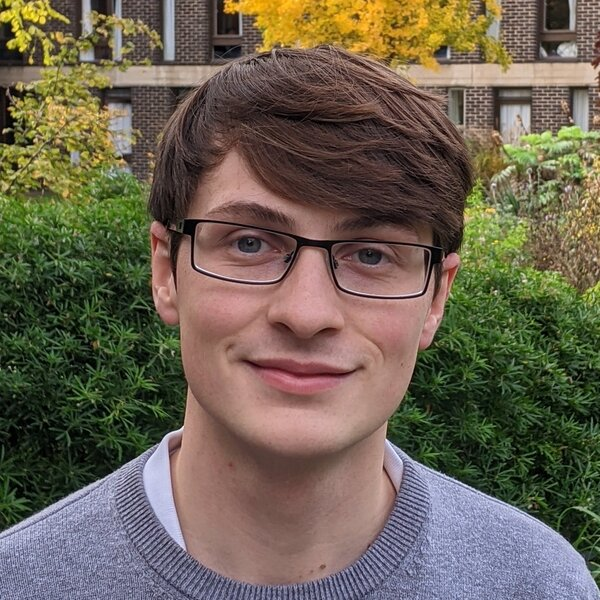
\includegraphics[width=0.1\textheight]{figures/students/thomas_gessey-jones.jpg}%
            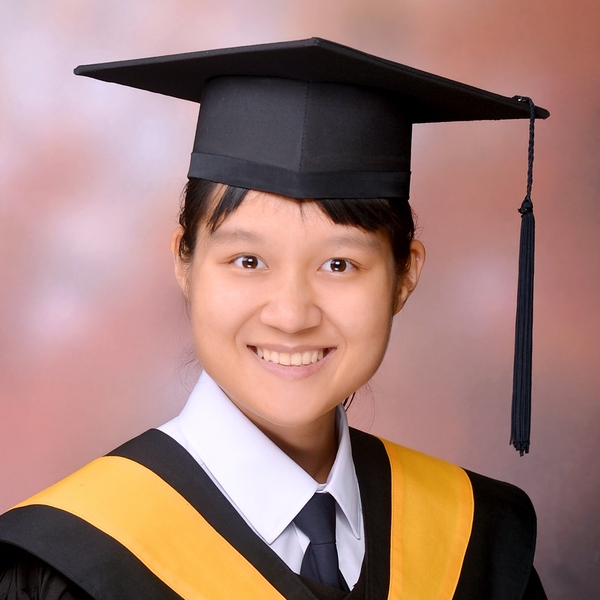
\includegraphics[width=0.1\textheight]{figures/students/wei-ning_deng.jpg}%
            %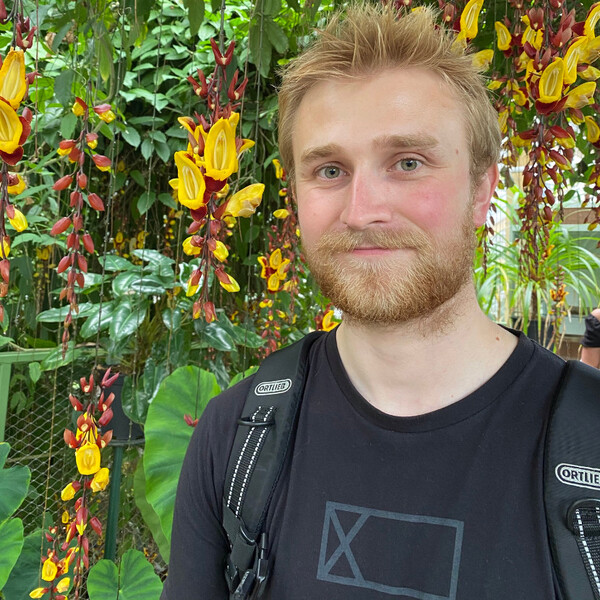
\includegraphics[width=0.1\textheight]{figures/students/will_barker.jpg}%
            %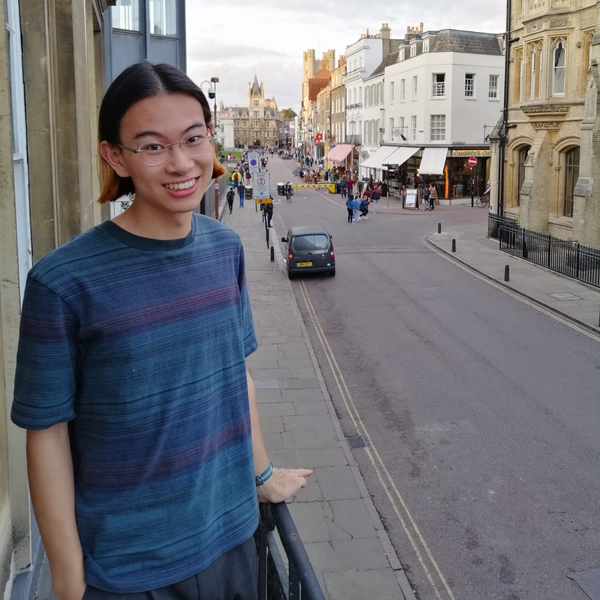
\includegraphics[width=0.1\textheight]{figures/students/zixiao_hu.jpg}%
    };
    \begin{enumerate}
        \item \texttt{anesthetic} \arxiv{1905.04768}
            \begin{itemize}
                \item how to get the most out of your nested sampling runs 
\item \texttt{\href{https://github.com/handley-lab/anesthetic}{github.com/handley-lab/anesthetic}}
            \end{itemize}
        \item \texttt{margarine} \arxiv{2207.11457}
            \begin{itemize}
                \item easy-to-use (neural) density estimation for marginal statistics
                \item \texttt{\href{https://github.com/htjb/margarine}{github.com/htjb/margarine}} 
            \end{itemize}
        \item \texttt{prescience} \arxiv{2309.06942}
            \begin{itemize}
                \item Fully Bayesian forecasts (no more need for Fisher)
                \item \texttt{\href{https://github.com/ThomasGesseyJones/FullyBayesianForecastsExample}{github.com/ThomasGesseyJones/FullyBayesianForecastsExample}} 
            \end{itemize}
        \item \texttt{unimpeded}
            \begin{itemize}
                \item up/downloading tool for transfering inference products (beyond chains)
                \item \texttt{\href{https://github.com/handley-lab/unimpeded}{github.com/handley-lab/unimpeded}} 
            \end{itemize}
    \end{enumerate}
\end{frame}
 
%\appendix
%\begin{frame}
%    \frametitle{A word on emulators: the dead measure}
%    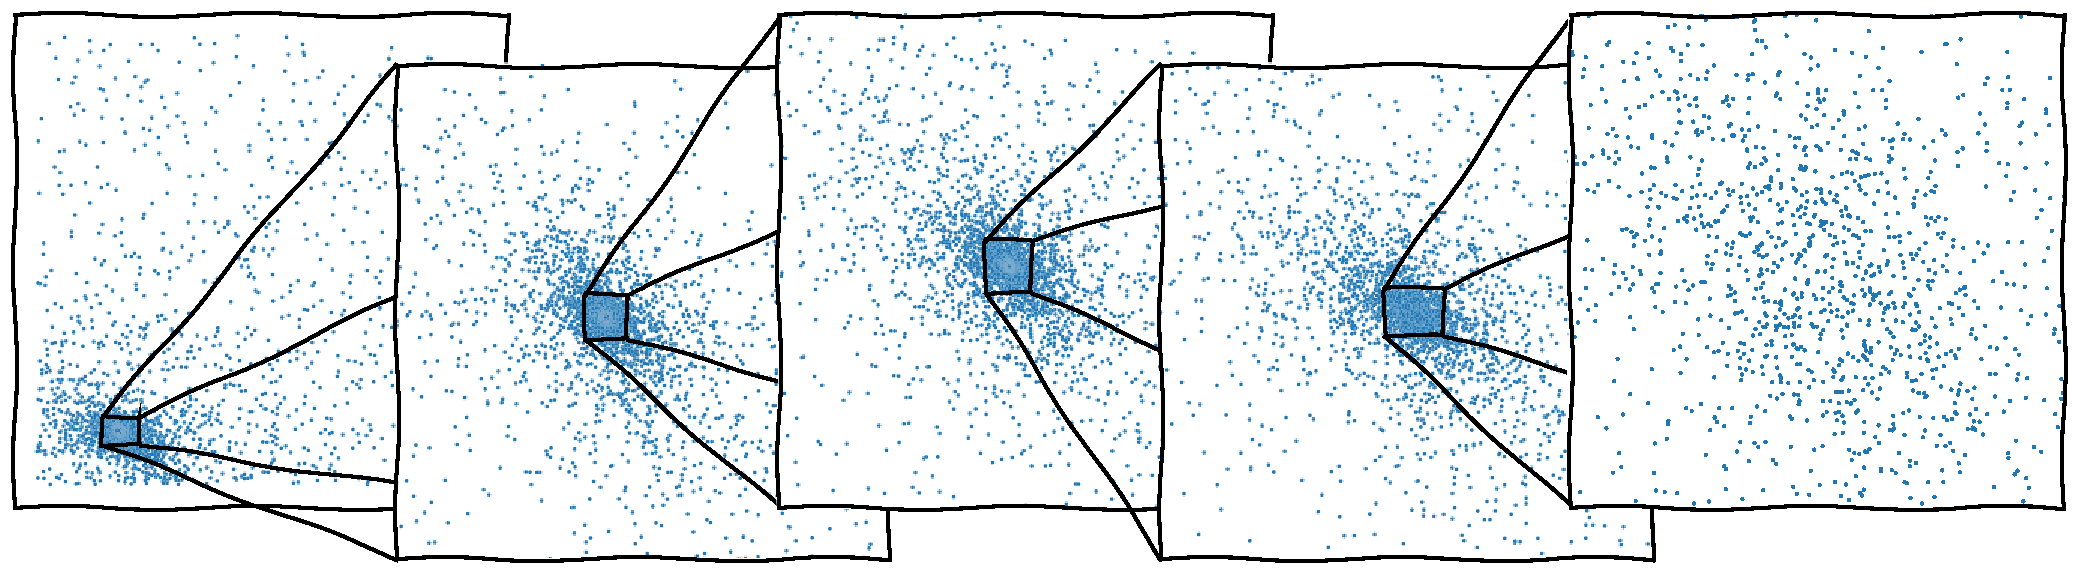
\includegraphics[width=\textwidth]{figures/dead_measure}
%    \begin{columns}
%        \column{0.69\textwidth}
%        \begin{itemize}
%            \item At the end, one is left with a set of discarded ``dead'' points.
%            \item Dead points have a unique scale-invariant distribution $\propto\: \tfrac{dV}{V}$.
%            \item Uniform over original region, exponentially concentrating on region of interest (until termination volume).
%            \item Good for training emulators (HERA~\arxiv{2108.07282}).
%        \end{itemize}
%        \column{0.3\textwidth}
%        \begin{block}{Applications}
%        \begin{itemize}
%            \item training emulators.
%            \item gridding simulations
%            \item beta flows
%            \item ``dead measure'' 
%        \end{itemize}
%        \end{block}
%    \end{columns}
%\end{frame}
\end{document}
